%%%%%%%%%%%%%%%%%%%%%%%%%%%%%%%%%%%%%%%%%%%%%%%%%%%%%%%%%%%%%%%%%%%%%%%%%%%%%%%%
%2345678901234567890123456789012345678901234567890123456789012345678901234567890
%        1         2         3         4         5         6         7         8

\documentclass[letterpaper, 10pt, conference]{ieeeconf}                             
\IEEEoverridecommandlockouts         % Needed if you want to use the \thanks command
                                                     
\overrideIEEEmargins                                                            


\usepackage{times} % assumes new font selection scheme installed
\usepackage{amsmath}
\usepackage{amssymb,longtable,calc}
\usepackage{mathptmx}
\usepackage[T1]{fontenc}                                                        
\usepackage[utf8]{inputenc}                                                     
\usepackage[english]{babel}                                                     
\usepackage{epsfig}                                                             
\usepackage{subfigure}                                                          
\usepackage{textcomp} %<- allows to use \textdegree but may overwrite           
                      %other settings                                           
\usepackage[textwidth=2cm,colorinlistoftodos]{todonotes} %add disable   
                                %to not show the todos                          
\usepackage{tikz}                                                               
\usetikzlibrary{arrows,positioning,fit,shapes,calc}
\usetikzlibrary{matrix}
\usepackage{flushend}                                                           
\usepackage{hyperref}  
\usepackage{amsmath}    

\usepackage[utf8]{inputenc}   
\usepackage[]{algorithm2e}
\usepackage{amsmath}


\usepackage{pgfplots} 
\usepackage{pgfplotstable}

\usepackage{cite}

% helper packages to work on the draft
\usepackage[tikz]{bclogo}
\usepackage{lipsum}

\usepackage{standalone}

\pgfplotsset{compat=newest}
\pgfplotsset{ 
  tick label style={font=\footnotesize}, 
  label style={font=\footnotesize}, 
  legend style={font=\footnotesize},
  title style = {font=\small}
}
\pgfplotscreateplotcyclelist{line style}{% 
  solid, mark options = {scale = .75}, every mark/.append style={fill=gray},mark=*\\% 
  densely dashed,mark options = {scale = .75},every mark/.append style={solid,fill=gray},mark=*\\% 
  densely dotted,mark options = {scale = .75},every mark/.append style={solid,fill=gray},mark=*\\% 
  dashed,mark options = {scale = .75},every mark/.append style={solid,fill=gray},mark=*\\% 
  dotted,mark options = {scale = .75},every mark/.append style={solid,fill=gray},mark=*\\% 
}
\pgfplotscreateplotcyclelist{bar style}{% 
  solid, fill=black!60!white\\%
  solid, fill=black!45!white\\%
  solid, fill=black!35!white\\%
  solid, fill=black!25!white\\%
}


\usepackage{xspace}
\makeatletter                                                                   
\DeclareTextCommandDefault{\textregisteredalt}{\footnotesize\textcircled{%      
      \check@mathfonts\fontsize\sf@size\z@\math@fontsfalse\selectfont R}}       
\DeclareRobustCommand\onedot{\futurelet\@let@token\@onedot}                     
\def\@onedot{\ifx\@let@token.\else.\null\fi\xspace}                             
\def\eg{e.g\onedot}                                                             
\def\ie{i.e\onedot}                                                             
\def\vgl{see }                                                                  
\def\Fig{Fig\onedot }                                                           
\def\Tab{Tab\onedot }                                                           
\def\Eq{Eq\onedot }
\def\Sec{Sec\onedot}                                                            
\def\etc{etc\onedot}                                                            
\def\etal{\textsl{et al}\onedot}                                                
\def\argmin{\mathop{\rm arg\,min}}                                              
\makeatother
                                                                    
\definecolor{lightGray}{rgb}{0.0,0.0,0.0}
\definecolor{kthColor}{RGB}{26,84,166}
                                                                                
\title{\LARGE \bf Feature Descriptors for Tracking by Detection: a Benchmark}                                                                               
                                                                                
                                                                                
\author{Alessandro Pieropan ~~~~ Mårten Bj{\"o}rkman  ~~~~ Niklas Bergstr{\"o}m ~~~~ Danica Kragic%
\thanks{The GPU used for this research was donated by the NVIDIA Corporation.}
\thanks{MB and DN are with CVAP/CAS, KTH, Stockholm, Sweden, {\tt celle,dani@kth.se}. AP, NB and MI are with the University of Tokyo, Japan, {\tt }.}}

\begin{document}                                                                
                                                                                
\maketitle                                                                      
\thispagestyle{empty}                                                           
\pagestyle{empty}



%%%%%%%%%%%%%%%%%%%%%%%%%%%%%% ABSTRACT %%%%%%%%%%%%%%%%%%%%%%%%%%%%%%%%%%%%%
\begin{abstract}
In this paper, we provide an extensive evaluation of the performance of local descriptors for tracking applications.
Many different descriptors have been proposed in the literature for a wide range of application in Computer Vision such as object recognition and 3D reconstruction. More recently, due to fast key-point detectors, feature descriptor can be used in online tracking frameworks. However, while much effort has been spent on evaluating their performance in terms of distinctiveness and robustness to image transformations, very little has been done in the contest of tracking. Our evaluation is performed in terms of distinctiveness, tracking precision and tracking speed. 

\end{abstract}

%%%%%%%%%%%%%%%%%%%%%%%%%%%%%% INTRODUCTION %%%%%%%%%%%%%%%%%%%%%%%%%%%%%%%%%%%
% \begin{}
\section{INTRODUCTION}
\label{sec:introduction}

Local regions of interest or key-point descriptors are widely used in Computer Vision for application such as object recognition and retrieval, 3D reconstruction and motion tracking. SIFT \cite{lowe04} is widely considered as one of the most robust feature descriptors, providing distinctiveness and invariance to common image transformations such as rotation and scale. However such a robustness comes with a computational cost. 

Recently there is much concern about efficiency caused mainly by two important factors. First there is a stable growth of portable camera enabled devices with limited computing power. Second, computer vision databases are steadily increasing in size. As a consequence, there is a growing interest within the computer vision community on fast key-point detectors and binary descriptors that can dramatically decrease the computational cost of detecting and matching local regions of interest. BRIEF \cite{calonder10} feature descriptor in combination with FAST \cite{rosten06} key-point detector is among the first attempts in this direction making it suitable for real time applications. However, despite the improvement in performance, BRIEF descriptor is not very robust to image transformations. This underlines the difficulty in finding a good compromise between two competing characteristics: distinctiveness and fast computation. 

More attempts has been done in this direction. BRISK \cite{leutenegger11} and ORB \cite{rublee11} propose some modification of the BRIEF and FAST in order to achieve scale and rotation invariance. The mentioned descriptors are faster that SIFT and have comparable matching precision with small image transformation. More recently the binary feature descriptor KAZE \cite{alcantarilla12} presented comparable results to SIFT on a standard dataset \cite{mikolajczyk05} designed to evaluate the robustness of local descriptors on several image transformations. Moreover, by using fast non linear filtering techniques Fast Explicit Diffusion \cite{goesele2010}, its accelerated version AKAZE \cite{alcantarilla13} could also beat SIFT in computational cost.\\
The main reason why AKAZE could outperform SIFT relies in the use of non linear filtering techniques. However, given the increasing use of GPUs in computer vision, it is not clear if such techniques can easily parallelizable on a GPU architecture as opposed to Gaussian filtering employed in SIFT. A recent work \cite{jiang2015} has shown that it is possible to deploy AKAZE descriptor on a specialized hardware and achieve a good speedup compared to the original implementation. By implementing the descriptor in CUDA we intend to analyze its performance using a GPU and compare it against the GPU implementations of their counterpart descriptors.

\missingfigure[figwidth=0.98\linewidth]{Intro figure showing tracker benchmark}

These extremely fast local descriptors not only improve the performance of vision tasks such as object retrieval and 3D reconstruction but they can be used in real-time tracking system. Yet, to the best of our knowledge, very little work has been done in evaluating key-points descriptor for the specific purpose of tracking. This work aims to target that issue by providing a fair and comprehensive evaluation of the most well known descriptors. We use the recall-precision measure to evaluate the matching distinctiveness of the features and we calculate the tracking precision by integrating each local descriptor in a key-point based tracker \cite{pieropan15}. Since there is no dataset designed to test local descriptors for tracking purposes , the videos used in the evaluation are gathered from well known tracking datasets described in \cite{wu2013,nebehay2014,hare2011}. We want to provide a practical guideline to binary descriptors for the specific task of tracking since it is not clear yet that a descriptor designed for image recognition is well suited for tracking.
 
The contribution of this work is four-fold:\\
\textbf{Dataset.} We collected 47 sequences from different public available datasets and annotated the ground-truth in a standardized format to ease the evaluation.\\
\textbf{Cuda Akaze.} Given the growing interest in the AKAZE feature descriptor and the lack of a GPU implementation, we provide our own using CUDA.\\
\textbf{Evaluation Library.} We integrated the most well known descriptors in a state-of-the-art key-point based 2D tracker and we provide an interface to enable the integration of new feature descriptors.\\
\textbf{Evaluation.}  There are three criteria the local descriptors are tested upon: distinctiveness, tracking precision and speed. First we measure the distinctiveness by matching the feature descriptors extracted in the first frame of the sequence and by computing the recall-precision. Then we calculate the low, medium and high tracking accuracy measures by integrating the descriptors in the 2D tracker. Last we profile the performance of each descriptor.

The dataset and all the code will be publicly available.


%\begin{figure}[t]
%	\vspace{2mm}
%\centerline{%
%	\subfigure[RGB-D video]{\includegraphics[width=0.48\linewidth]{images/intro/intro_rgb.png}}
%	%\includegraphics[width=0.48\linewidth]{images/intro/intro_disp.png}\label{fig:intro_rgbd}}}
%	%\centerline{%
%	\subfigure[Audio]{\includegraphics[width=0.48\linewidth]{images/intro/audio_intro.png}\label{fig:intro_audio}}}
%	%subfigure[Objects pose]{\includegraphics[width=0.48\linewidth]{images/intro/intro_track.png}\label{fig:intro_objects}}}
%\caption{An RGB-D video modality and an audio modality give complementary information about an observed human action. This is a motivation of why to use a recognition method that takes both modalities into account.}
%\vspace{-3mm}
%\label{fig:intro}
%\end{figure}


%% %%%%%%%%%%%%%%%%%%%%%%%%%%% RELATED WORK %%%%%%%%%%%%%%%%%%%%%%%%%%%%%%%% 
\section{Related Work}
\label{sec:relatedwork}

Assessing the performance of various computational techniques and providing the suitable benchmarks for these receives increasing attention in several areas  \cite{christensen02} COMMENT\footnote{We need more references here and more recent ones  benchmarks in robotics etc}. The need for evaluating feature descriptors in terms of object recognition, classification and alike is clearly important. One of the most relevant work has been done more than a decade ago by Mikolajczyk et al. \cite{mikolajczyk05} where affine region detectors are evaluated in terms of repatability and accuracy. SIFT feature descriptor \cite{lowe04} and its extension GLOH \cite{mikolajczyk05} showed the best performance on the dataset decribed in \cite{mikolajczyk2005b}. More recently, due to a stable increase of portable devices and large scale databases, there is more focus being 
put on the computational cost and runtime requirements of such descriptors. For example, SURF \cite{bay2008} is among the first descriptors that presented lower computational requirements than SIFT and comparable precision. More recently, Calonder et al. \cite{calonder10} proposed to use a binary descriptor BRIEF, as opposed to SIFT histogram, in combination with a fast corner detector FAST \cite{rosten06} achieving a fraction of the runtime performance to SURF. However, the descriptor has comparable results only when small transformations are applied to an image since it is not scale or rotation invariant. 

The ORB descriptor (Oriented Fast and Rotated Brief) proposed by Rublee et al. \cite{rublee11} enhances BRIEF adding the rotation invariance. Another binary descriptor, BRISK \cite{leutenegger11}, provides both scale and orientation invariance. Its corner detector, AGAST \cite{mair2010}, is also faster also faster than FAST. However, its invariance properties influence the overall performance.
Heinly et al. \cite{heinly2012} conducted an extensive evaluation of these three binary descriptors using SURF and SIFT as a baseline on the Oxford dataset \cite{mikolajczyk2005b}. As expected, SIFT demonstrated the most precise performance while BRIEF was the fastest one. However, since BRIEF is not rotation and scale invariant, its performance is significantly inferior in cases of significant image transformations. This just supports the fact that optimizing between precision and speed is not so trivial.  In the area of robotics, the low computational cost of an employed feature descriptors may have the high impact in real-time applications such as visual servoing, simultaneous mapping and localization (SLAM), and alike. 

Recently, a promising binary feature descriptor, KAZE, has been proposed by Alcantarilla et al. \cite{alcantarilla12}. The main strength of the descriptor lies in using non linear diffusion filtering techniques \cite{weickert98} to build the scale space as opposed to Gaussian blurring. Since the latter smooths without distinction at any scale, it does not preserve object boundaries. On the other hand, non-linear diffusion filtering techniques preserve edges, resulting in an increased distinctiveness of the feature descriptor. Once again, an improved precision comes at a cost of speed. However, by using the Fast Explicit Diffusion \cite{goesele2010}, an accelerated version of the feature descriptor AKAZE \cite{alcantarilla13} was proposed. AKAZE achieves better accuracy than SIFT and has a lower computational cost. The experiments have been performed on the Oxford dataset, designed to evaluate the precision of feature descriptors under various image transformations. Such feature descriptors are now employed in real-time system such as tracking by detection \cite{nebehay2014,pieropan15,pieropan15b} and  SLAM \cite{murartal2015}. 



%% %%%%%%%%%%%%%%%%%%%%%%%%%%% DATASET AND EVALUATION DESCRIPTION %%%%%%%%%%%%%%%%%%%%%%%%%%%%%%%%
%\input{dataset}

%% %%%%%%%%%%%%%%%%%%%%%%%%%%% BENCHMARK %%%%%%%%%%%%%%%%%%%%%%%%%%%%%%%%
\section{Benchmark}

The purpose of the experiments conducted are three-fold. First we want to measure the descriptiveness of the feature descriptors for matching purposes, this is crucial for the recovery of a tracker upon object loss. Second we measure the tracking accuracy by integrating each feature descriptor in our 2D tracker and compute the overlap measure using the estimated object position. Third we profile each separate step required in tracking by detection (key-point detection, descriptor computation and feature match) in order to evaluate the performance of the feature descriptors for real-time frameworks.

\subsection{Dataset}

\begin{figure*}[t]
	\vspace{2mm}
\centerline{%
	\subfigure{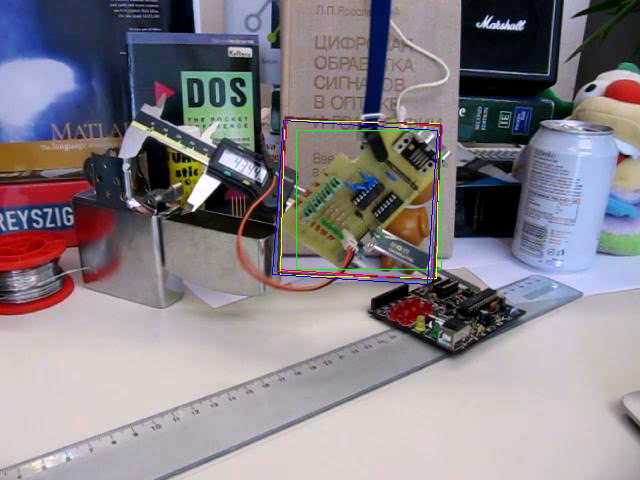
\includegraphics[width=0.19\linewidth]{imgs/dataset/d1.png}}
	\subfigure{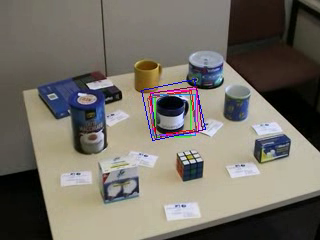
\includegraphics[width=0.19\linewidth]{imgs/dataset/d2.png}}
	\subfigure{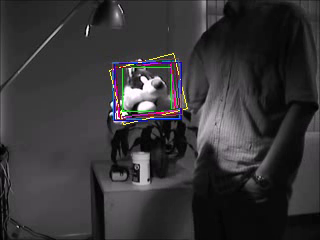
\includegraphics[width=0.19\linewidth]{imgs/dataset/d3.png}}
	\subfigure{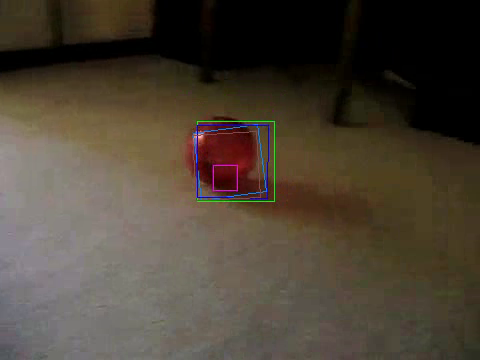
\includegraphics[width=0.19\linewidth]{imgs/dataset/d4.png}}
	\subfigure{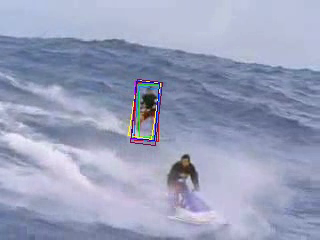
\includegraphics[width=0.19\linewidth]{imgs/dataset/d5.png}}}
	\vspace{-2mm}
\centerline{%
	\subfigure{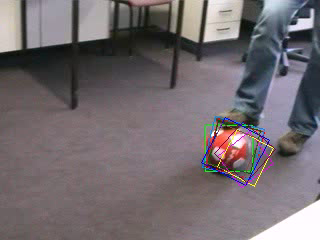
\includegraphics[width=0.19\linewidth]{imgs/dataset/d6.png}}
	\subfigure{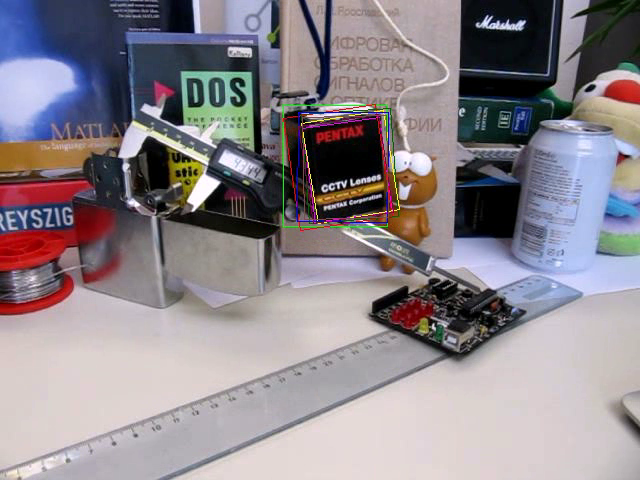
\includegraphics[width=0.19\linewidth]{imgs/dataset/d7.png}}
	\subfigure{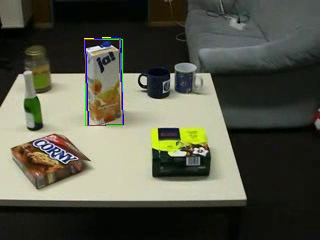
\includegraphics[width=0.19\linewidth]{imgs/dataset/d8.png}}
	\subfigure{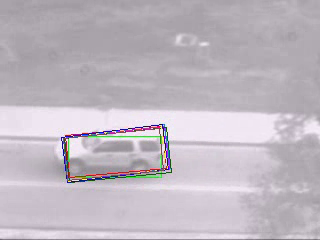
\includegraphics[width=0.19\linewidth]{imgs/dataset/d9.png}}
	\subfigure{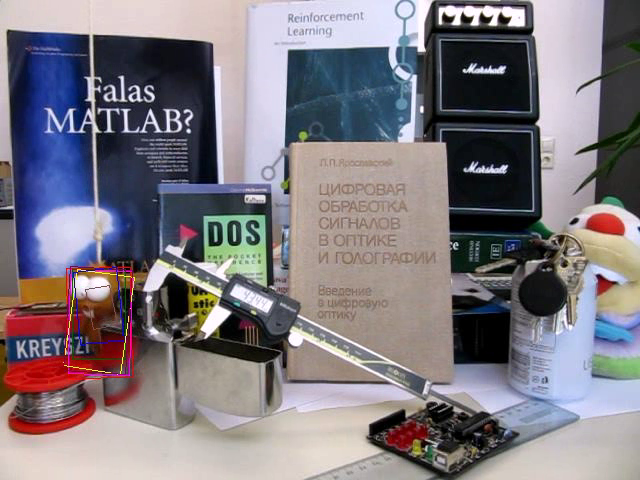
\includegraphics[width=0.19\linewidth]{imgs/dataset/d10.png}}}
\caption{The sequences of the dataset includes both indoor and outdoor scenarios with different light conditions.}
\vspace{-3mm}
\label{fig:data_example}
\end{figure*}


There are many publicly available datasets designed for tracking, however there is disagreement on how the data are stored. In order to facilitate the evaluation we collected the videos of different datasets and standardized how the data are stored. Fig.~\ref{fig:data_example} shows some examples. Each video is stored as a sequence of images while the ground truth, represented by an oriented bounding box, is saved in a comma separated value file where each row correspond to an image frame and contains 8 values representing the pairs x,y of each vertex of the box. The dataset will be available publicly, along with all the code to perform the experiments and compute the evaluation.

\subsection{Matching Evaluation Criteria}

\begin{figure}[b]
	%\vspace{-2mm}
	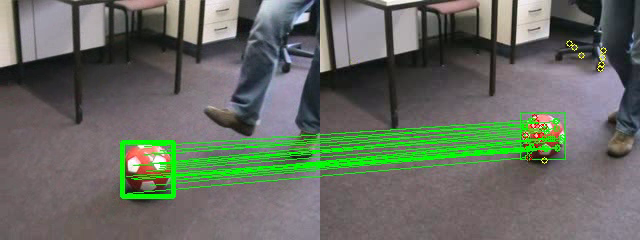
\includegraphics[width=0.95\linewidth]{imgs/matching.png}
\vspace{-2.5mm}	
\caption{Example showing how the matching precision is calculated. the image n the right shows the initial frame of the sequence. Matches in green are true positives. Circles in red are false positives. Yellow circles are false negatives, feature descriptors that are inside the object in the current frame but have a match with the background in our model.}
\label{fig:matching}
\end{figure}

Given as sequence of images $I_{1},...,I_{n}$ and the bounding box ground truth $gb_{1},...,gb_{n}$, we extract the set of target key-points descriptors $K_{1}$ from the first image of the sequence and we label all the key-points within $gb_{1}$ as descriptors of the object. For any subsequent image key-points $K_{t}$ are extracted and matched with $K_{1}$, generating a list of matches $M(i,j)_{k}$, where \textit{i} indicates a key-point descriptor of our target set $K_{1}$, and \textit{j} a descriptor of our test set. the test set is then labeled as follows:

\begin{equation}
K_{t}^{j} = 
\begin{cases}
\text{true positive}  \text{ if } K_{t}^{j} \in gb_{n} \land K_{1}^{i} \in gb_{1} \\
\text{false positive}  \text{ if } K_{t}^{j} \notin gb_{n} \land K_{1}^{i} \in gb_{1} \\
\text{false negative}  \text{ if } K_{t}^{j} \in gb_{n} \land K_{1}^{i} \notin gb_{1} \\
\end{cases}
\end{equation}

where the pair \textit{i,j} is determined by the matching result $M(i,j)_{k}$. Fig.~\ref{fig:matching} shows an example of how the key-points are labeled. The average ratio of true positives underlines the ability of a tracker to find the object and potentially recover from track loss. False negatives are feature descriptors that appear in the current frame but have no corresponding match in the initial test set $K_{1}$. This may happen due to drastic change in appearance of the object. The ratio of false positives is very important to consider since it indicates the average number of outliers that will be used to estimate the pose of the object, resulting in a bad pose estimation without employing additional filtering techniques. One widely used filtering technique consists in discarding all matched key-points if the ratio between the score of the best match and the second best match is below a certain threshold $\rho$. We define a key-point as ambiguous, if this criteria is not met. The  number of ambiguous true and false positives is then calculated to evaluate the distinctiveness of the descriptors and evaluate the influence of this common filtering technique on the results.

\subsection{Evaluating tracking precision}
\label{sec:accuracy}

\begin{algorithm}[h]
 \KwData{$I_{1},...,I_{n},b_{1}$}
 \KwResult{$b_{2},...,b_{n}$}
 $K_{1} \gets$ \textbf{extract\_points}($I_{1},b_1$)\;
 \For{$i \gets 2 : n$}{
   $K_{i}^{*} \gets$ track\_points($K_{i-1},I_{i-1},I_i$)\;
   $b_i \gets$ estimate\_pose($K_{i}^{*}$)\;
   $K_{i}' \gets$ \textbf{extract\_points}($I_{i},b_i$)\;
   $M \gets$ \textbf{match\_points}($K_{1},K_{i}'$)\;
   $K_{i} \gets$ merge\_keypoints($K_i^* ,  M$)\;
 }
 \caption{\label{alg:algorithm}Overview of the tracking algorithm used to compute the precision. The feature descriptors are employed in the steps in bold. }
\end{algorithm}

In order to measure the precision of the feature descriptors for tracking we employ a sparse key-point based tracker. The tracker requires a bounding box in the initial image of a sequence as initialization to extract feature descriptors that represent the \textit{model} of the object to track. The algorithm estimates the position of the object, represented as an oriented bounding box, with a combination of sparse optical flow and feature matching as shown in Alg.~\ref{alg:algorithm}. The original algorithm used ORB. We upgraded our algorithm making it more modular and able to cope with any possible feature descriptor. To estimate the precision we used the widely accepted overlap measure:

\begin{equation}
	\Theta (b_{t}, b_{gt}) = \frac{b_{t} \cap b_{gt}}{b_{t} \cup b_{gt}}
\end{equation}

where \textit{$b_{t}$} is the bounding box estimated by our tracker and
\textit{$b_{gt}$} is the bounding box provided by the ground truth. We define 
three precision requirements $\Upsilon$ (0.25, 0.5, 0.75) that indicates low, medium and high tracking accuracy. This is a more indicative evaluation compared to the overall accuracy. For instance, an overall value of 0.5 is ambiguous because it may indicate either a stable average accuracy around the value or a very precise evaluation in part of the video while poor in the rest.

The estimated object box \textit{$b_{t}$} is considered a true positive (TP) for a defined threshold of
accuracy $\Upsilon$ if:

\begin{equation}
\begin{cases}
b_{t} = TP  \text{ if } \Theta(b_{t}, b_{gt}) > \Upsilon \\
b_{t} = FP  \text{ otherwise }\\
\end{cases}
\end{equation}

The overall accuracy of the tracker for each precision requirement is calculated as:

\begin{equation}
\text{recall } = \frac{TP}{\text{TP } + \text{ FN}}
\end{equation}

%\missingfigure[figwidth=0.98\linewidth]{Figure showing the estimated bounding boxes and the ground truth to show the different behavior of trackers}

\subsection{Parameter setting}

All the descriptors require many parameters in order t be initialized properly. In order to evaluate the most fair comparison between them we decided to keep the values suggested by the original author of the descriptor or the implementation. However, there are some parameters that most of the feature descriptors shares that we set to the same value. The maximum number of features extracted is set to 2500 and the number of octaves is set to 4.





%% %%%%%%%%%%%%%%%%%%%%%%%%%%% CONCLUSION %%%%%%%%%%%%%%%%%%%%%%%%%%%%%%%%
\section{Conclusion}

We proposed an evaluation of the most common feature descriptors for the purpose of tracking by detection. Our experiments have shown that most of the feature descriptors have comparable results. While AKAZE and SIFT have proven to be more distinctive, ORB and BRISK compensate their weak descriptors with a higher number of points extracted. Given the growing interested in AKAZE descriptor we provided a GPU implementation so that it can be used for real time system. The code to perform the benchmark, the dataset and our implementation of AKAZE will be publicly available in order to ease researches in this area.




\bibliographystyle{unsrt}
\bibliography{ref}

\end{document}
